% Intended LaTeX compiler: pdflatex
\documentclass[../main]{subfiles}


\begin{document}

\section{Bias-Variance tradeoff}
\label{sec:org18aabf8}
\subsection{Bias-Variance tradeoff nel Machine Learning}
\label{sec:org4c5d15f}

Si consideri un dataset \(D=\set{(x_{i},z_{i})\mid i =1,\dots,N}\), si consideri una \href{20250624155858-neurone_artificiale.org}{rete neurale} con \href{20250624155858-neurone_artificiale.org}{output} \(f_{\bm{w},b}(t)\) dipendente dai parametri \(\bm{w},b\), e se ne consideri il \href{20250627110009-training_error_and_test_error.org}{processo di addestramento} tramite \href{20250627153729-condizioni_necessarie_per_l_esistenza_di_un_minimo_di_una_funzione_reale.org}{minimizzazione} della \href{20250624155858-neurone_artificiale.org}{funzione costo}\footnote{Vedi \href{20250710141709-mean_square_error.org}{Empirical MSE}}
\begin{equation*}
\frac{1}{N}\sum_{i=1}^{N} (z_{i}- f_{\bm{w},b}(x_{i}))^{2}.
\end{equation*}

Si divide quindi il dataset \(D\) negli insiemi di training \(\mathscr{T}\) e di test \(\mathrm{T}\). Ciascuna possibile scelta di \(\mathscr{T}\) produce, tramite minimizzazione, una funzione \(f_{\mathscr{T}}\coloneqq f_{\bm{w}^{*},b^{*}}\).

Fissato dunque \((x_{0},z_{0}) \in D\), si vuole calcolare in che modo varia l'errore commesso in quel punto in relazione alla scelta di \(\mathscr{T}\):
\begin{equation*}
\media_{\bm{w},b}\left[\left(z_{0}-f_{\bm{w},b}(x_{0})\right)^{2}\right].
\end{equation*}
dove la media è calcolata al variare dei parametri \(\bm{w},b\) (il variare dei parametri è equivalente al variare di \(\mathscr{T}\)).

Per semplicità si omettono le variabili e i parametri. Si noti che l'unica cosa che dipende dai parametri è \(f_{\bm{w},b}\).
\begin{align*}
\media\left[(z_{0} - f)^2\right]
&= \media\left[(z_{0} - \media[f] + \media[f] - f)^2\right] \\
&= \media\left[(z_{0} - \media[f])^2 + (f - \media[f])^2 + 2(z_{0} - \media[f])(\media[f] - f)\right] \\
&= \media\left[(z_{0} - \media[f])^2\right]
   + \parentesi{\mathrm{Var}(f)}{\media\left[(f - \media[f])^2\right]}
   + \media\left[2(z_{0} - \media[f])(\media[f] - f)\right] \\
&= (z_{0} - \media[f])^2 + \mathrm{Var}(f) + 2(z_{0} - \media[f]) {\media\left[\media[f] - f\right]}\\
&= (z_{0} - \media[f])^2 + \mathrm{Var}(f) + 2(z_{0} - \media[f]) \cancel{\left(\media[f] - \media [f]\right)}\\
&= (z_{0} - \media[f])^2 + \mathrm{Var}(f) \\
&= \mathrm{Var}\left(f_{\bm{w},b}\right) + \left(z_{0} - \media[f_{\bm{w},b}]\right)^2
\end{align*}
dove \(\left(z_{0} - \media[f_{\bm{w},b}]\right)\) è il bias.

Se il modello è molto flessibile (ovvero si può adattare molto bene ai dati), allora
\begin{equation*}
z_{0}\approx \media[f_{\bm{w},b}].
\end{equation*}
Allo stesso tempo la varianza è molto alta, in quanto basta modificare di poco il training set affinché la funzione di output (adattandosi molto ai dati) cambi tanto.

Viceversa, se il modello è poco flessibile, allora difficilmente \(\left(z_{0} - \media[f_{\bm{w},b}]\right)\) è piccolo; allo stesso tempo, cambiando di poco il training set, la funzione di output non cambia molto, e dunque la varianza è bassa.

Pertanto le due parti si comportano come mostrato in figura~\ref{fig:biasvarianceml}

\begin{figure}
\begin{center}
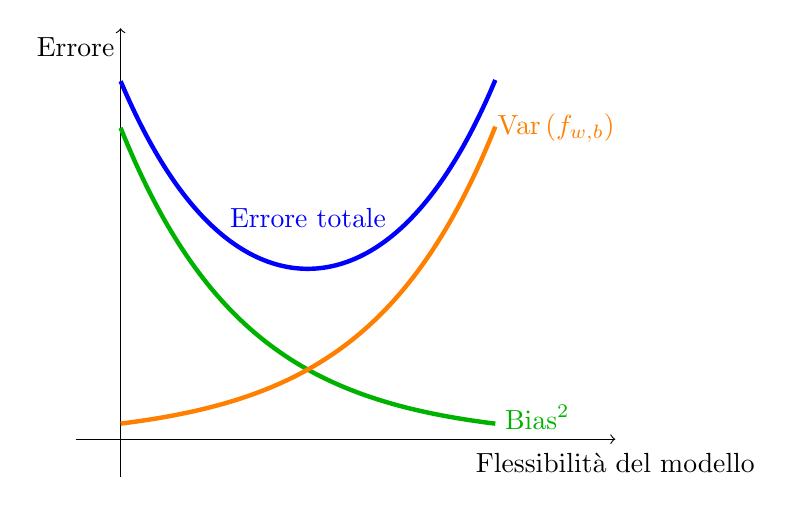
\begin{tikzpicture}
\begin{axis}[
    axis lines=middle,
    xlabel={Flessibilità del modello},
    ylabel={Errore},
    xlabel style={at={(1,0)}, anchor=south, yshift=-2pt},
    ylabel style={at={(0,1)}, anchor=north},
    xmin=0, xmax=12,
    ymin=0, ymax=12,
    xtick=\empty,
    ytick=\empty,
    enlargelimits=true,
    legend pos=north west,
    legend style={draw=none},
    axis line style={->}
]

% curva decrescente (verde)
\addplot[
    domain=0:10,
    samples=100,
    smooth,
    ultra thick,
    green!70!black
] {10*exp(-0.3*x)};
% curva crescente (arancione)
\addplot[
    domain=0:10,
    samples=100,
    smooth,
    ultra thick,
    orange
] {0.5*exp(0.3*x)};
% curva totale (blu)
\addplot[
    domain=0:10,
    samples=100,
    smooth,
    ultra thick,
    blue
] {0.5*exp(0.3*x)+10*exp(-0.3*x)+1};

% Etichetta per la curva decrescente
\node[anchor=west, green!70!black] at (10,0.7) {$\mathrm{Bias}^{2}$};

% Etichetta per la curva crescente
\node[anchor=west, orange] at (9.8,10) {$\mathrm{Var}\left(f_{\bm{w},b}\right)$};

% Etichetta per il totlae
\node[anchor=south, blue] at (5,6.5) {Errore totale};

\end{axis}
\end{tikzpicture}
\end{center}
\caption{\label{fig:biasvarianceml}Errore nell'approssimazione di un dataset}
\end{figure}
\end{document}
